\section{Описание реализации программы} {
    После чтения сцены из файла иницилизируется структура,
    хранящая все данные для отрисовки.
    В этот процесс входит иницилизация трассировщика
    и построениетеневых буферов для источников.
    В результате получается структура данных трассировщика,
    объединяющая в себе всё необходимое для получения цвета какого-либо пиксля.
    всё, что нужно для трассировки лучей.
    Трассировщик хранит буферы источников, так как с их помощью вычисляется
    яркость каждой следующей точки, что рассматривается как часть процесса
    трассировки.
    Также в нём содержатся лучи, которые нужно трассировать для того, чтобы
    получить цвет каждого пикселя.
    Каждый луч представляет собой массив из сегментов луча, на которые
    он делится при столкновении с объектом.
    
    Затем запускается трассировка лучей.
    Трассировщик хранит матрицу размерности изображения, содержащую
    лучи, которые следует трассировать для получения цвета пиеселя.
    Выполняется проход по этой матрице с определённым шагом.
    Если пиксель не расчитан, то отслеживается ход соответствующего луча,
    после чего вычисляется его итоговый цвет.

    После того, как все нужные пиксели получены, они отображаются.
    Для этого выполняется 2 действия: извлечение пикселей,
    масштабирование изображения и его отрисовка.
    Трассировщик содержит данные о каждом расчитаном пикселе.
    Сделовательно, их цвета нужно извлечь и поместить в
    структуру данных изображения.
    Изображение, которое получается после очередного процесса трассировки,
    по размеру меньше ожидаемого, так как вычисляются пиксели с шагом.
    Таким образом, его размер нужно увеличить до нужного.
    После того: как картинка сфоритрована, она передаётся
    графической карте (GPU) и отображается на экране.

    Далее шаг отрисовки должен уменьшиться.
    Для этого он либо делится на 2, либо уменьшается на 1.
    Если шаг равен 1, то последующей трассировки не требуется
    и алгоритм завершается.
    Седуюшее срабатывание алгоритма визуализации произойдёт
    при изменении сцены.
    
    Схема алгоритма визуализации сцены представлена на рисунке \ref{fig:idefs}.

    \begin{figure}[H]
    	\centering
    	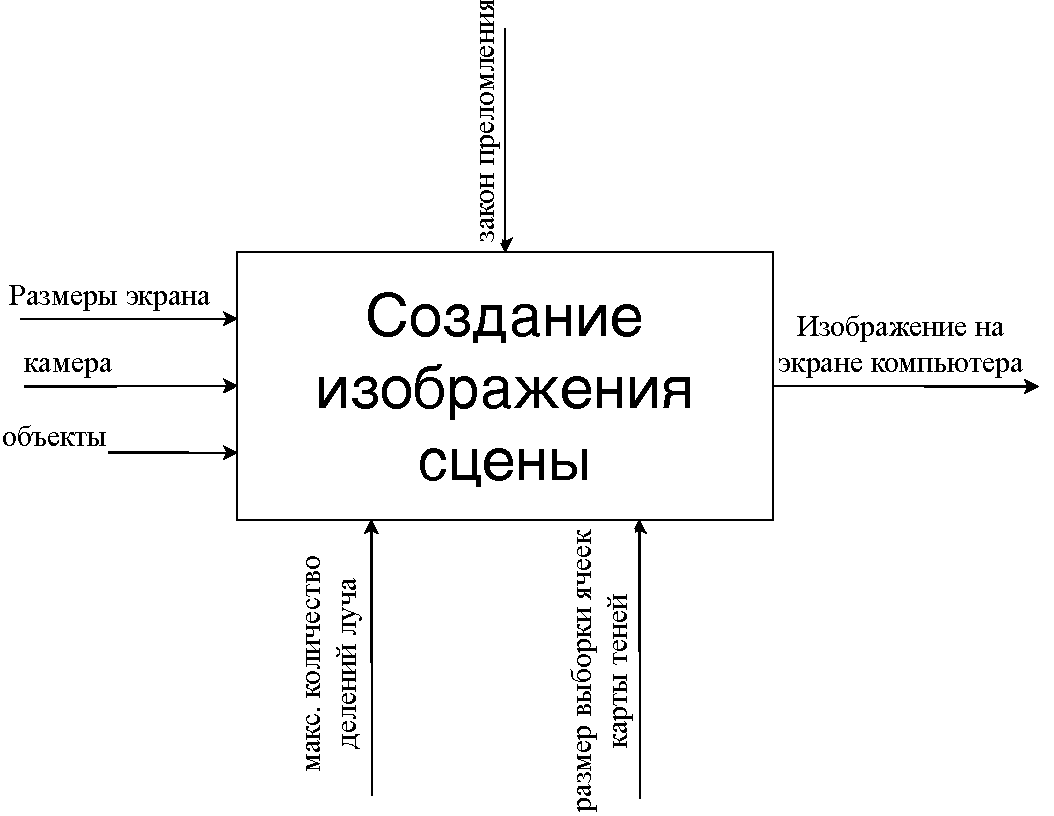
\includegraphics[height=0.5\textheight]{img/idef0.pdf}
        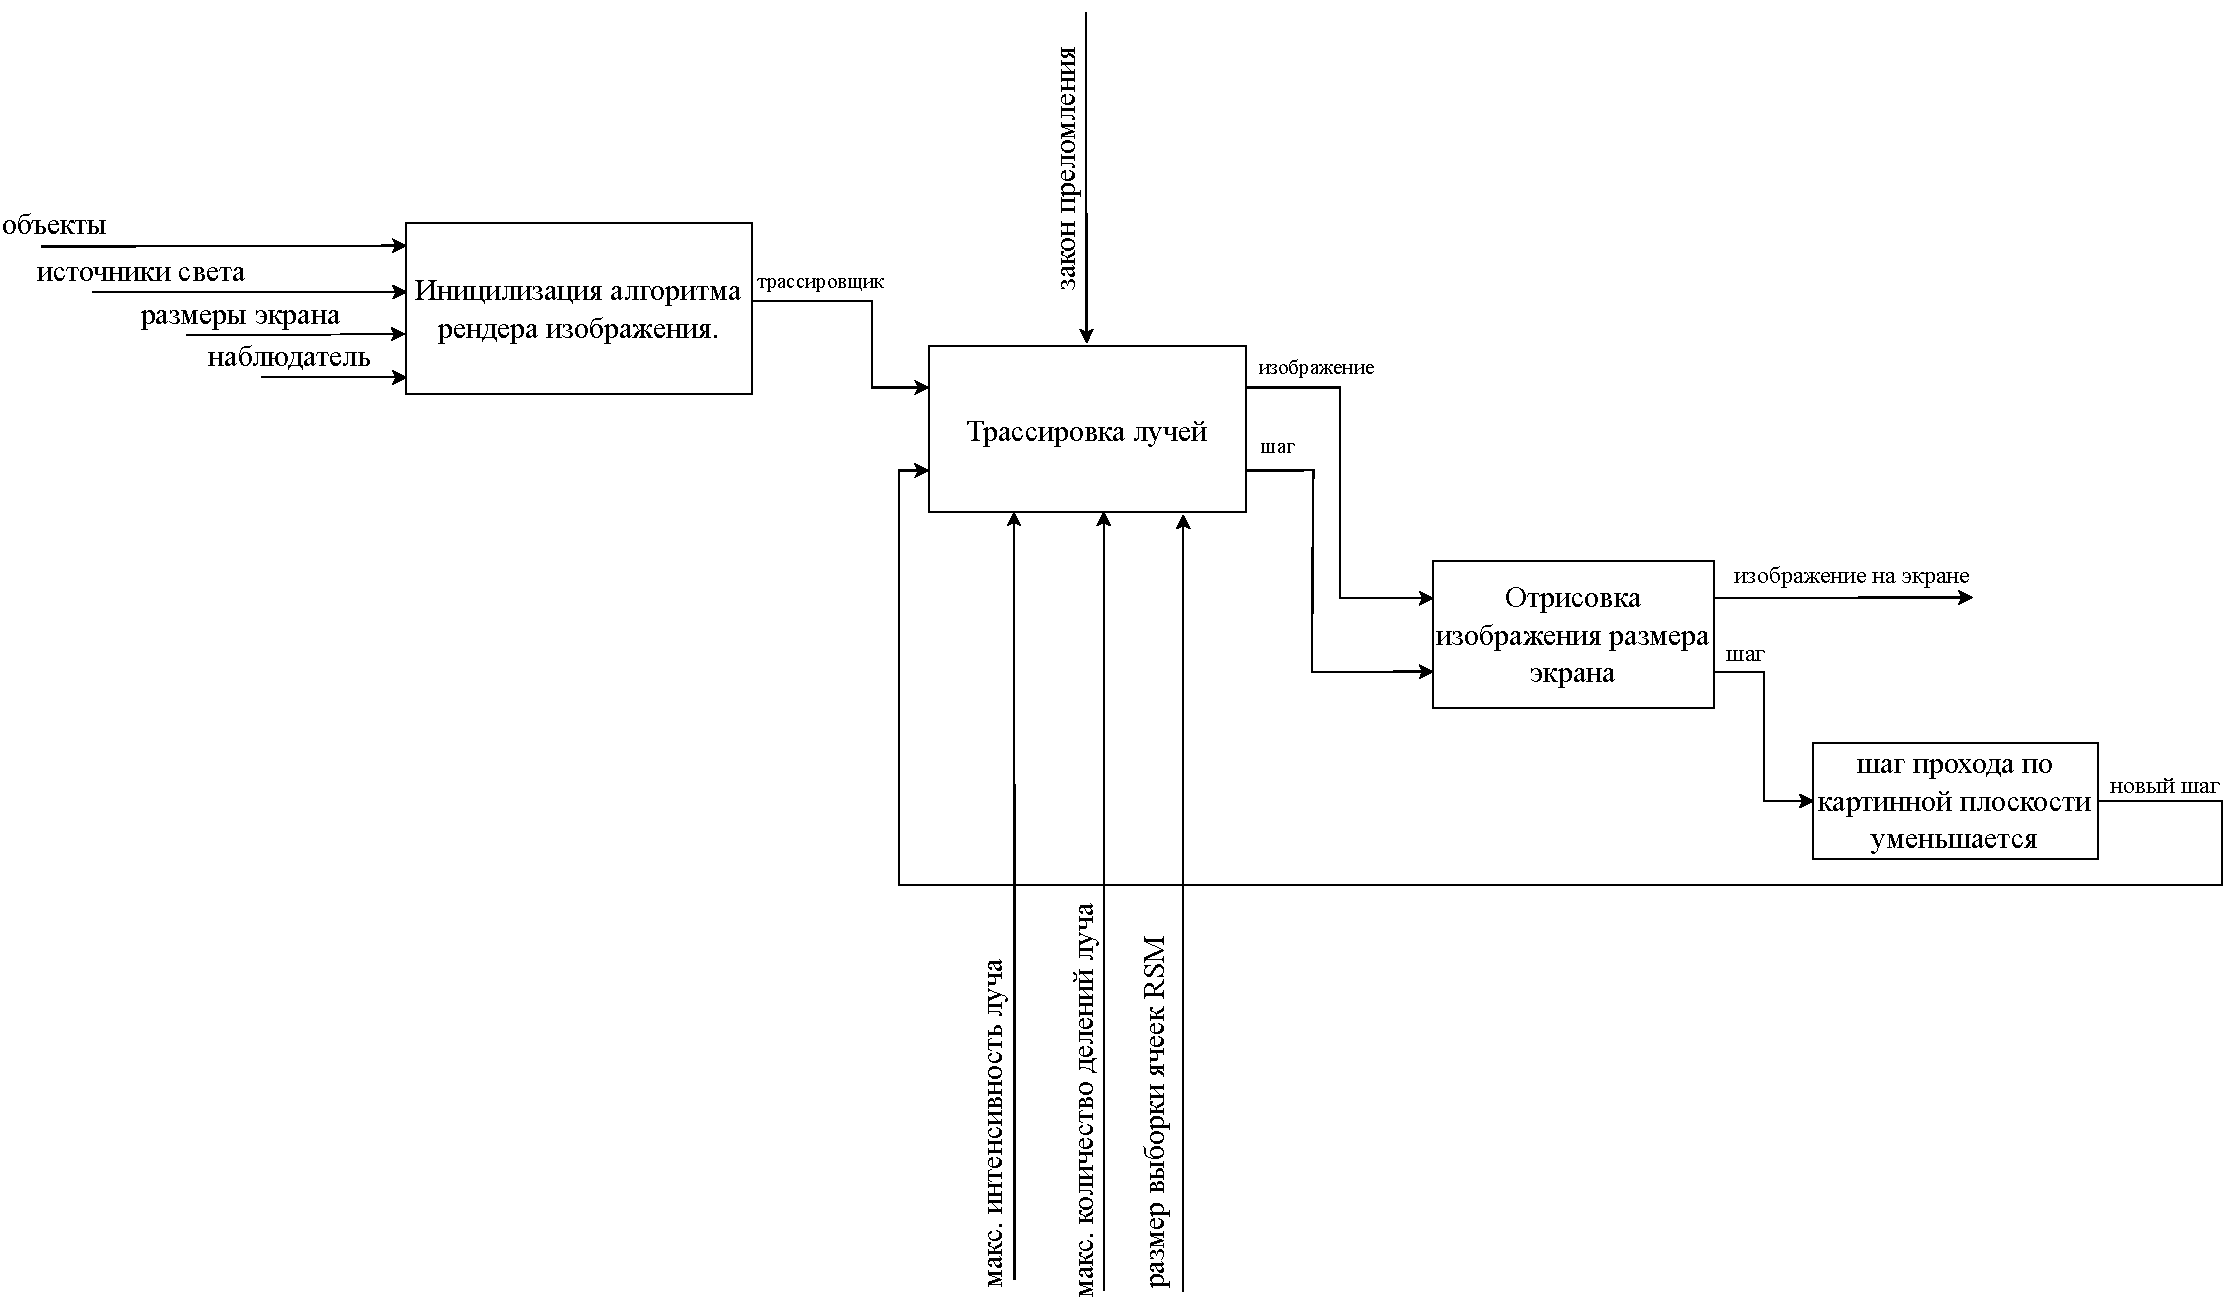
\includegraphics[width=0.99\textwidth]{img/idef1.pdf}
    	\caption{Idef диаграмма алгоритма визуализации сцены уровней 0, 1}
    	\label{fig:idefs}
    \end{figure}

    \vspace{5cm}
    На рисунках \ref{fig:trace1}--\ref{fig:trace2} предствлены
    схемы алгоритмов трассировки.

    \begin{figure}[H]
    	\centering
    	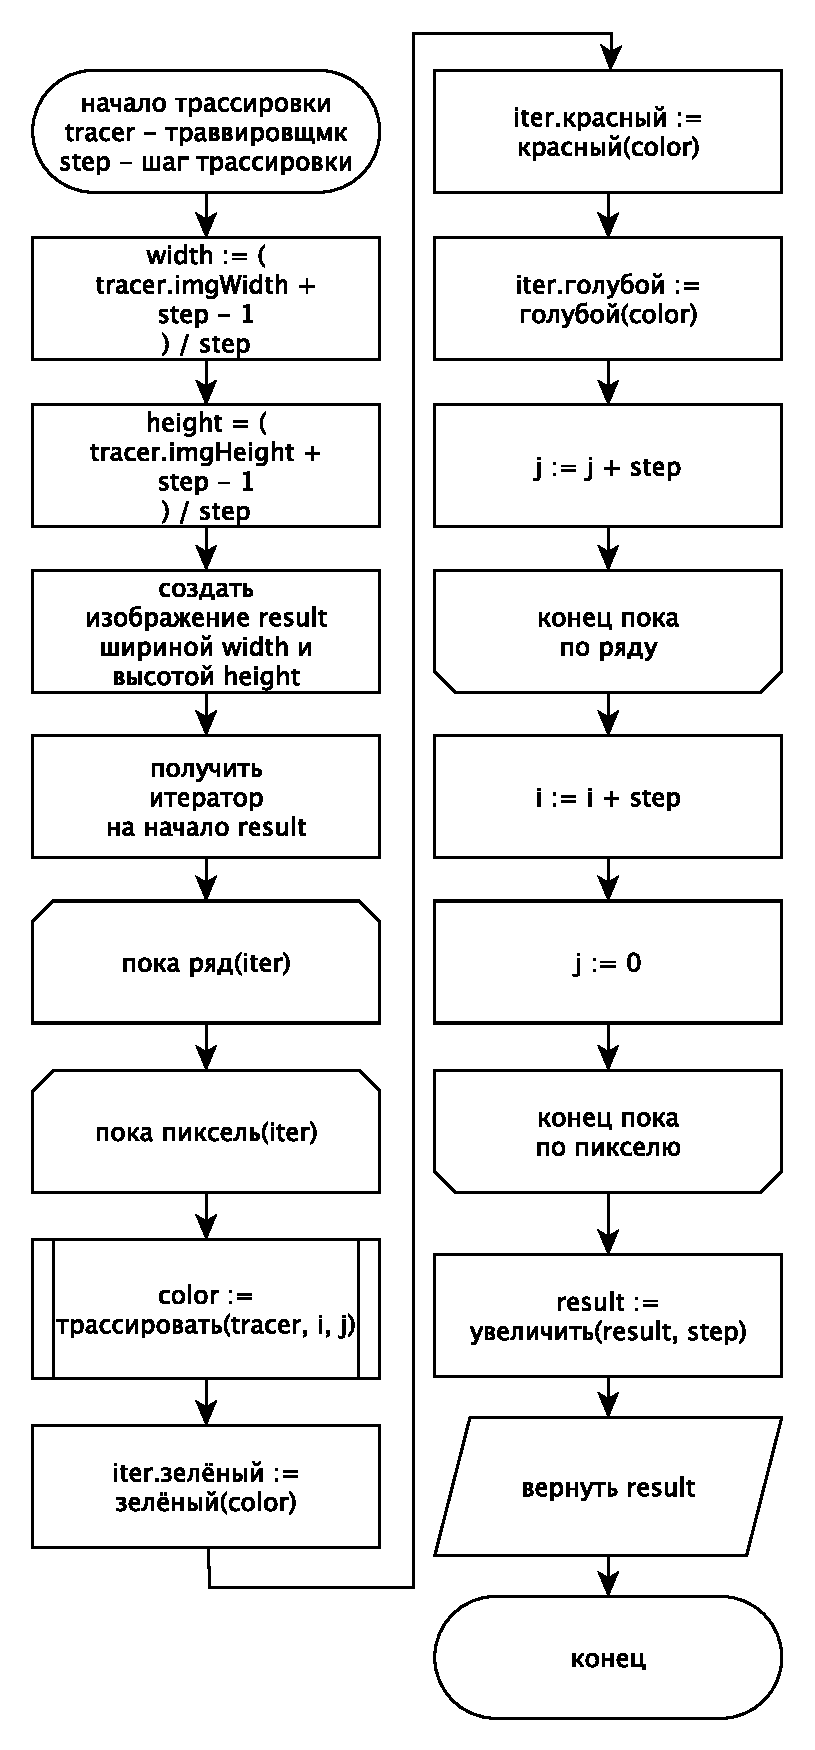
\includegraphics[height=0.9\textheight]{img/trace1.pdf}
    	\caption{Схема алгоритма трассировки лучей с заданным шагом}
    	\label{fig:trace1}
    \end{figure}

    \begin{figure}[H]
    	\centering
    	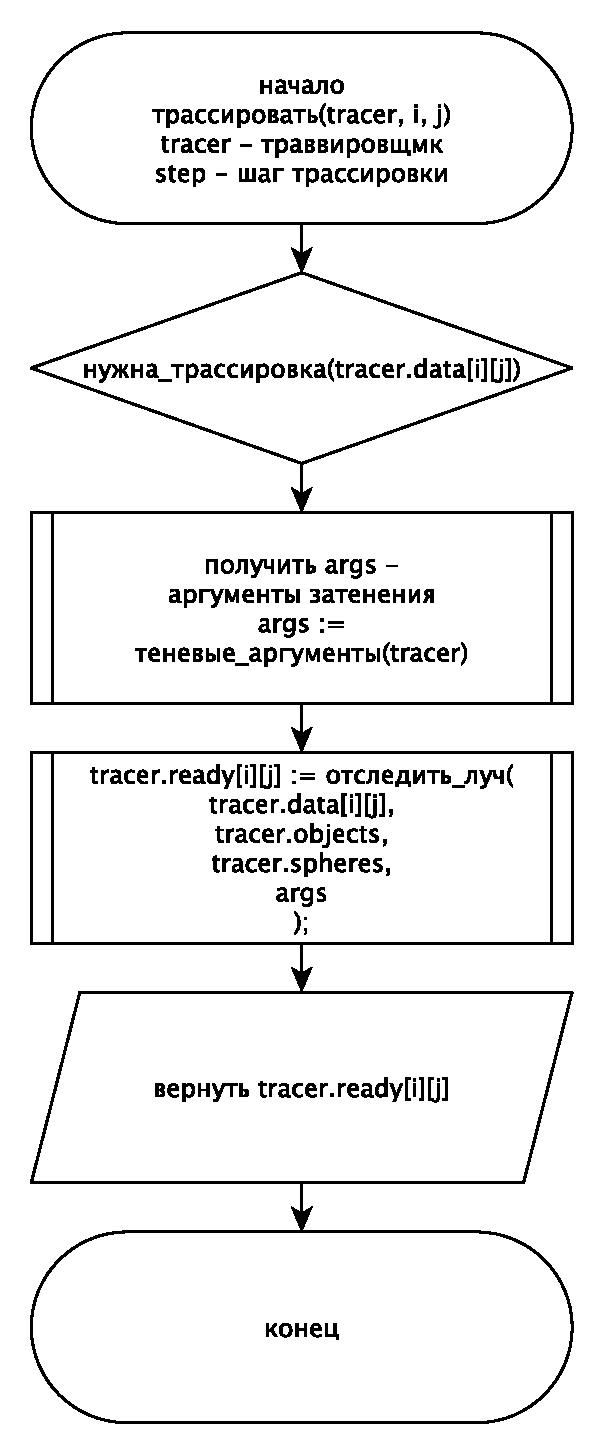
\includegraphics[height=0.5\textheight]{img/trace2.pdf}
    	\caption{Схема алгоритма трассировки для получения цвета пикселя}
    	\label{fig:trace2}
    \end{figure}
}